% % % % % % % % % % % % % % % % % % % % % %
% Präambel
% % % % % % % % % % % % % % % % % % % % % %

\documentclass[paper = a4, fontsize = 12pt, parskip = half]{scrartcl} % Doku: "scrguide"
\usepackage[ngerman]{babel} % Sprachenunterstützung für LaTeX; Doku: "gerdoc"7
\usepackage[T1]{fontenc} % Schriftkodierung
\usepackage[utf8]{inputenc} % Eingabekodierung
\usepackage{lmodern} % Schrift: Latin Modern

\usepackage{scrlayer-scrpage}
\usepackage{microtype} % mikrotypographische Erweiterungen von pdfTeX; s.a. microtype-DE
\usepackage{amsmath} % AMSmath-Paket der American Mathematical Society (AMS)
\usepackage{eurosym} % das Euro-Zeichen (?) z.B. mit \EUR{}
\usepackage{grffile} % erweiterte Unterstützung für Grafikdateinamen (z.B. mehrere Punkte)
\usepackage{graphicx} % Einbinden von Grafiken; Doku: "grfguide"
\usepackage{url} % Querverweise können im Text hervorgehoben werden
\usepackage{hyperref} % Querverweise in Hyperlinks umwandeln
\usepackage{setspace} % Ermöglicht Änderungen des Zeilenabstands
\usepackage{paralist} % Erweiterung der Listenumgebungen\usepackage{hyperref}
\usepackage{csquotes} % advanced facilities for inline and display quotations
\usepackage{wrapfig} % Grafiken mit Text umfließen
\usepackage{color}
\usepackage{listings}

\usepackage[style=ieee]{biblatex}
\addbibresource{library.bib}

\hypersetup{pdfborder={0 0 0}}
\setkomafont{captionlabel}{\small\sffamily\bfseries}
\addtokomafont{caption}{\small}

% custom commands to uniformly style XML ELEMents and ATTRibutes
% also inclusion of style to brush up XML listings with syntax highlighting and line-numbers
\usepackage{listings}
\usepackage{color}
 
\definecolor{dkgreen}{rgb}{0,0.6,0}
\definecolor{gray}{rgb}{0.5,0.5,0.5}
\definecolor{mauve}{rgb}{0.58,0,0.82}
\definecolor{gray}{rgb}{0.4,0.4,0.4}
\definecolor{darkblue}{rgb}{0.0,0.0,0.6}
\definecolor{lightblue}{rgb}{0.0,0.0,0.9}
\definecolor{cyan}{rgb}{0.0,0.6,0.6}
\definecolor{darkred}{rgb}{0.6,0.0,0.0}


\lstset{
  basicstyle=\ttfamily\footnotesize,
  columns=fullflexible,
  showstringspaces=false,
  numbers=left,                   % where to put the line-numbers
  numberstyle=\tiny\color{gray},  % the style that is used for the line-numbers
  stepnumber=1,
  numbersep=5pt,                  % how far the line-numbers are from the code
  backgroundcolor=\color{white},      % choose the background color. You must add \usepackage{color}
  showspaces=false,               % show spaces adding particular underscores
  showstringspaces=false,         % underline spaces within strings
  showtabs=false,                 % show tabs within strings adding particular underscores
  frame=none,                   % adds a frame around the code
  rulecolor=\color{black},        % if not set, the frame-color may be changed on line-breaks within not-black text (e.g. commens (green here))
  tabsize=2,                      % sets default tabsize to 2 spaces
  captionpos=b,                   % sets the caption-position to bottom
  breaklines=true,                % sets automatic line breaking
  breakatwhitespace=false,        % sets if automatic breaks should only happen at whitespace
  title=\lstname,                   % show the filename of files included with \lstinputlisting;
                                  % also try caption instead of title  
  commentstyle=\color{gray}\upshape
}


\lstdefinelanguage{XML}
{
  morestring=[s][\color{mauve}]{"}{"},
  morestring=[s][\color{black}]{>}{<},
  morecomment=[s]{<?}{?>},
  morecomment=[s][\color{dkgreen}]{<!--}{-->},
  stringstyle=\color{black},
  identifierstyle=\color{lightblue},
  keywordstyle=\color{red},
  morekeywords={xmlns,xsi,noNamespaceSchemaLocation,type,id,x,y,source,target,version,tool,transRef,roleRef,objective,eventually}% list your attributes here
}
\def\attr#1{\texttt{#1}}
\def\elem#1{\texttt{\textbf{#1}}}
\lstnewenvironment{lstcode}
                    {\lstset{frame=shadowbox, linewidth=10cm}}{}

%% set heading and footer
%% scrheadings default: 
%% footer - middle: page number
\pagestyle{scrheadings}
%%\automark[subsection]{section}
%% user specific
%% usage:
%% \position[heading/footer for the titlepage]{heading/footer for the rest of the document}
%% heading - left
% \ihead[]{}
%% heading - center
% \chead[]{}
%% heading - right
% \ohead[]{}
%% footer - left
% \ifoot[]{}
%% footer - center
% \cfoot[]{}
%% footer - right
% \ofoot[]{}

% % % % % % % % % % % % % % % % % % % % % %

\begin{document}
% % % % % % % % % % % % % % % % % % % % % %
% Beginn der Titelseite 
% % % % % % % % % % % % % % % % % % % % % %

\begin{titlepage}

	\begin{center}
		
\includegraphics[width=8cm]{images/logo_aau.png} \\
		\vspace{8mm}
		\huge\textbf{Alpen-Adria-Universität Klagenfurt} \\
		\vspace{3mm}
		Fakultät für Technische Wissenschaften \\
		\vspace{3mm}
		Institut für Informationstechnologie (ITEC)\\
		\vspace{3mm}
	\end{center}

	\vspace{5mm}

	\begin{center}
		\textbf{Lehrveranstaltung: \\
			Seminar aus Angewandte Informatik} \\
		\vspace{2mm}
		LV-Leiter: Univ.-Prof. Dipl.-Ing. Dr. Hermann Hellwagner \\
		LV-Nr.: 622.000 \\
		SS 2021
	\end{center}

	\vspace{15mm}

	\begin{center}
		\Large\textbf{MPEG-DASH Standard} \\
		\vspace{2mm}
		\normalsize Dynamic Adaptive Streaming over HTTP
	\end{center}

	\vspace{40mm}

	\begin{flushleft}
		\textbf{Andreas Kogler} \\
		E-Mail: andrkogler@edu.aau.at \\
		Studienrichtung: Bachelorstudium Angewandte Informatik \\
		Matrikel-Nr.: 11702050\\
		Datum: \today
	\end{flushleft}

\end{titlepage}

% % % % % % % % % % % % % % % % % % % % % %

% % % % % % % % % % % % % % % % % % % % % % 
% Inhalts- und Abbildungsverzeichnis
% % % % % % % % % % % % % % % % % % % % % %

% \thispagestyle{empty}
\tableofcontents
\listoffigures
% \listoftables
\pagebreak

% % % % % % % % % % % % % % % % % % % % % %

% % % % % % % % % % % % % % % % % % % % % % 
% Beginn des Dokuments
% % % % % % % % % % % % % % % % % % % % % %

% \newpage
\setcounter{page}{1}
\onehalfspacing

\section*{Abstract}
Wie der jährlich herausgegebene Cisco Visual Networking Index \cite{cisco_syst_inc_cisco_2017} zeigt, steigt der Anteil von Videodaten im Internet rapide. Mit Ende 2021 sollen Videodaten 80\% des globalen Gesamtdatenvolumens ausmachen \cite{cisco_syst_inc_cisco_2017}.

Das vormals verbreitete \textit{Real-Time Transport Protocol} operiert unter der Annahme eines \textit{Managed}-IP-Netzwerks, wohingegen in modernen Umgebungen Content Distribution Networks (CDNs) verwendet werden \cite{sodagar_mpeg-dash_2011}. Während in Managed-IP-Netzwerken Server für die Verteilung der (Video-)Daten fest vorgegeben sind, können sich Server in CDNs dynamisch aufgrund einer Reihe von Kennzahlen regelmäßig ändern \cite{buyya_content_2008}. Um diesem Problem und der Vielfalt an proprietären Streamingstandards zu entgegnen, hat MPEG einen Standard für \textit{Dynamic Adaptive Streaming over HTTP}, auch bekannt als MPEG-DASH, entwickelt \cite{sodagar_mpeg-dash_2011}.

Im Mittelpunkt steht dabei die dynamische Bitratenadaptierung der Videodaten je nach verfügbarer Bandbreite von Netzwerk und Endgerät. Da sich die verfügbare Bandbreite während der Wiedergabe des Videos ändern kann, müssen verschiedene Algorithmen zur dynamischen Selektion der Bitrate angewandt werden \cite{bentaleb_survey_2019}.

Die eigentlichen Audio- und Video-Bitströme werden dabei in kleinere Segmente unterteilt, welche wiederum in verschiedenen Qualitätsstufen für den Client zur Auswahl stehen. Jedes Segment besitzt eine eindeutige URL, über die es mittels HTTP GET-Request angefragt werden kann. Alle verfügbaren Segment-URLs werden in der \textit{Multimedia Presentation Description (MPD)} angegeben. Durch Einlesen dieser XML-Datei am Anfang des Streamingprozesses, lernt der Client über alle verfügbaren Segmente und Qualitätsstufen und kann diese gemäß des verwendeten Algorithmus auswählen \cite{sodagar_mpeg-dash_2011}.

MPEG-DASH definiert in seiner Spezifikation lediglich die Segmentformate, den Aufbau der MPD-Datei und die verpflichtende Verwendung von HTTP/1.1 \cite{mpeg_dynamic_2013}. Viele weitere Aspekte wie beispielsweise Austausch der MPD, Codierung der Daten oder Verhalten bei der Bitratenadaption sind Gegenstand der jeweiligen Implementierung \cite{sodagar_mpeg-dash_2011}.

Diese Arbeit bietet einen Überblick zu MPEG-DASH allgemein, legt ihren Schwerpunkt jedoch auf durch den Standard vorgegebene Aspekte.
Nicht-standardisierte Teile werden konzeptuell eingeführt und anhand aktueller Lösungsbeispiele konkretisiert. Für Details wird an den jeweiligen Stellen auf tiefergehende Lektüre verwiesen.

\section{Warum Adaptives Streaming?}
Potentielle Endgeräte, mit denen Menschen Videostreams konsumieren, erfreuen sich großer Diversität. Neben klassischen Medien wie PC und TV-Receiver haben sich vor allem Smartphones, Tablets und Spielkonsolen in verschiedensten Konfigurationen im täglichen Gebrauch der NutzerInnen etabliert.

Diese Endgeräte weisen unterschiedliche Charakteristiken auf, welche die Anforderungen an das Videoformat und dessen Übertragung stark beeinflussen. Vorrangig betrachten wir im Kontext von Videostreaming die Bildschirmgröße und Auflösung sowie die verfügbare Bandbreite des Endgeräts und des Netzwerks.
Es reicht also nicht, ein Video in einer einzigen Version serverseitig zu speichern. Während die Qualität für einen Full-HD Computerbildschirm völlig ausreichend sein könnte, würde sie auf einem 4k-TV aufgrund zu geringer Auflösung verschwommen angezeigt werden und wäre für einen Smartphone-Bildschirm unnötig groß. Letzteres lässt bereits vermuten, dass auch die effiziente Nutzung von Netzwerkressourcen eine zentrale Rolle im Videostreaming spielt.

Smartphones, die mit steigender Tendenz einen Großteil des globalen Internetverkehrs ausmachen, sind zu einem Großteil über das Mobilfunknetz an das Internet angebunden \cite{cisco_syst_inc_cisco_2017}. Hier kann es insbesondere zu Schwankungen in der verfügbaren Bandbreite am Endgerät und im Netzwerk kommen. Ein Einbruch der verfügbaren Bandbreite führt zu clientseitigen Ladezeiten bei der Wiedergabe, was die QoE (Quality of Experience) wiederum stark negativ beeinflusst \cite{seufert_survey_2015}.

Diese Umstände und der wachsende Markt führten schließlich zur Idee des adaptiven Videostreamings. Ein Konzept, in dem die Bitrate des zu übertragenden Videos während der Wiedergabe dynamisch an die Netzwerkgegebenheiten angepasst (adaptiert) wird. Das führt bei Netzwerkengpässen zwar dazu dass Teile des konsumierten Videos mit geringerer Qualität wiedergegeben werden, vermeidet allerdings gefürchtete Unterbrechungen der Medienwiedergabe und beeinträchtigt die QoE für den Benutzer merklich weniger \cite{seufert_survey_2015}.

\section{Adaptive-Streaming-Standards - Überblick}
Adaptives Streaming ist ein generelles Konzept und keine konkrete Technologie. Zur konkreten Umsetzung haben sich in den letzten Jahren zwei große Standards gebildet. Einerseits wurde von Apple das vormals proprietäre\footnote{mittlerweile als Internet-Standard unter RFC 8216 \cite{pantos_http_nodate} verfügbar} Protokoll HLS (HTTP Live Streaming) entwickelt, während die Moving Pictures Expert Group (MPEG) den offenen Standard MPEG-DASH (Dynamic Adaptive Streaming over HTTP) entwickelt hat. Der DASH-Standard wurde 2012 offiziell von MPEG unter der ISO/IEC-Nummer 23009 \cite{international_organization_for_standardization_isoiec_nodate} veröffentlicht und besteht aus acht Teilen:

\begin{itemize}
	\item \textbf{Part 1:} Media Presentation Description and Segment Formats
	\item \textbf{Part 2:} Reference Software and Conformance
	\item \textbf{Part 3:} Implementation Guidelines
	\item \textbf{Part 4:} Format Independent Segment Encryption and Authentication
	\item \textbf{Part 5:} Server and Network Assisted DASH (SAND)
	\item \textbf{Part 6:} DASH with Server Push and WebSockets
	\item \textbf{Part 7:} Delivery of CMAF Content with DASH
	\item \textbf{Part 8:} Session based DASH Operation
\end{itemize}

HLS wurde 2009 von Apple veröffentlicht und wird im RFC 8216 \cite{pantos_http_nodate} der IETF beschrieben.

Beide Technologien setzen für die Übertragung auf der Applikationsebene das Hyper Text Transfer Protocol (HTTP) ein. Beide Protokolle werden von einer weiten Palette an Endgeräten unterstützt. Ausnahme ist die Unterstützung bei Apple Geräten. Der Safari-Browser, welcher bei iPhone und iPad als Standard ausgeliefert wird, unterstützt nativ kein MPEG-DASH \cite{timmerer_live_2015} .

\section{Einführung in MPEG-DASH}
Um adaptives Streaming via MPEG-DASH zu ermöglichen, wird die Mediendatei zunächst in mehrere, kleine Segmente zwischen zwei und zehn Sekunden Länge aufgeteilt \cite{international_organization_for_standardization_isoiec_nodate}. Jedes dieser Segmente wird anschließend in verschiedenen Qualitätsstufen kodiert. Segmente in einer höheren Qualitätsstufe benötigen mehr Speicherplatz und später auch mehr Bandbreite bei der Übertragung. Die so entstandenen Segmente werden schließlich auf einen Webserver hochgeladen, wo sie mittels HTTP GET-Requests angefragt werden können \cite{sodagar_mpeg-dash_2011}. 

Clientseitig übernimmt DASH-konforme Software die Kommunikation mit dem Webserver. Um dem Client einen Überblick über die verfügbaren Qualitätsstufen des angefragten Videos zu bieten, wird vom Server zu Beginn die \textit{Media Presentation Description}, kurz \textit{MPD}, bereitgestellt. Ein Teil der Clientsoftware misst permanent die zur Verfügung stehende Bandbreite und bestimmt so, in welcher Qualitätsstufe ein Segment angefragt wird. Dieser Teil der Software wird \textit{Bitrate Adaptation Algorithm} genannt \cite{bentaleb_survey_2019}. 

	\begin{figure}
		\centering
		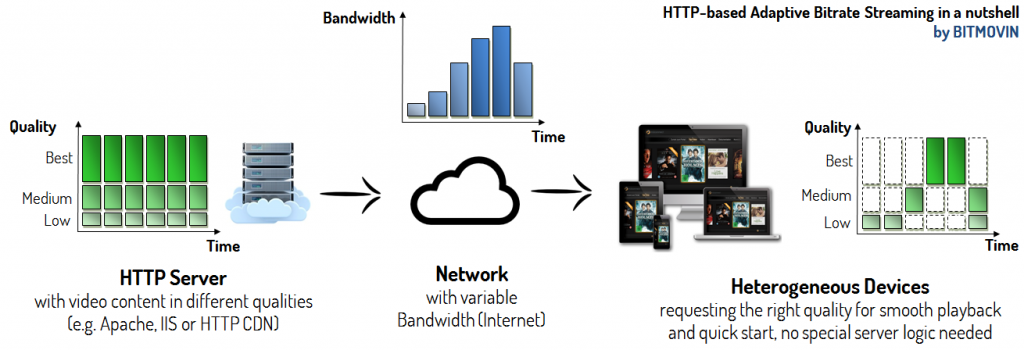
\includegraphics[width=14cm]{images/adaptive-streaming-basic.png}
		\caption{Überblick HTTP Adaptive Streaming, Quelle: \hyperref{https://bitmovin.com/dynamic-adaptive-streaming-http-mpeg-dash/}{}{}{Bitmovin}}
	\end{figure}


\subsection{Media Presentation Description (MPD)}
Bevor der Streamingprozess beginnt, muss die MPD zwischen Client und Server ausgetauscht werden. Der Austauschprozess wird dabei nicht vom Standard vorgegeben, sondern ist von der Implementierung des jeweiligen Anbieters abhängig \cite{sodagar_mpeg-dash_2011}.

Eine MPD-Datei dient als \textit{Inhaltsverzeichnis} für den Client, bietet einen Überblick über sämtliche vorhandene Mediendaten (Video, Audio, Untertitel), deren Eigenschaften und die zugehörigen URLs an die HTTP-Requests gestellt werden, um das jeweilige Segment zu erhalten \cite{international_organization_for_standardization_isoiec_nodate}.

Die Dateistruktur wird strikt durch den Standard vorgegeben. MPD-Dateien folgen einem durch den Standard vorgegebenen XML-Schema. Abbildung \ref{mpd_components} veranschaulicht die wichtigsten Komponenten einer MPD, auf die in den kommenden Abschnitten näher eingegangen wird.

	\begin{figure}[ht]
		\centering
		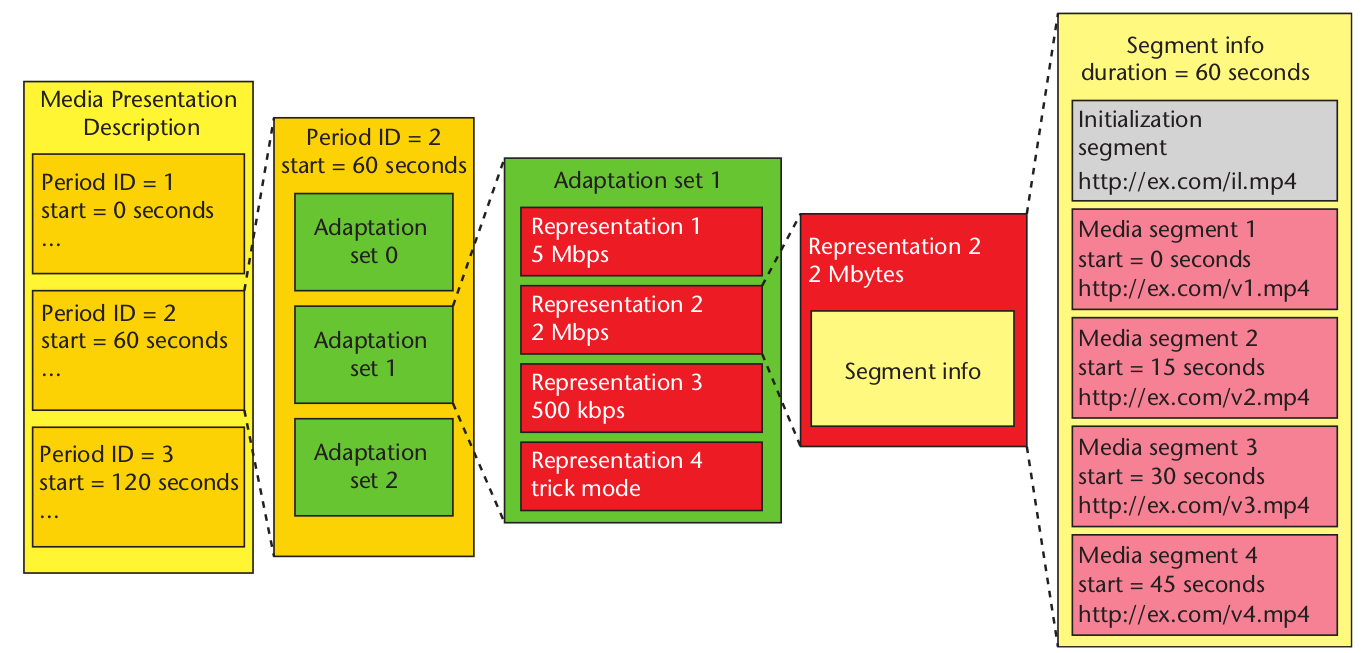
\includegraphics[width=12cm]{images/mpd-structure.png}
		\caption{Gliederung einer MPD, Quelle: \cite{sodagar_mpeg-dash_2011}, Figure 3, S. 65}
		\label{mpd_components}
	\end{figure}

\textbf{Notiz:} Es werden pro Abschnitt nur Attribute und Sub-Elemente besprochen die laut ISO/IEC 23009-1 als \textit{Mandatory}, also unbedingt notwendig, gekennzeichnet sind oder dem Zweck eines anschaulichen Beispiels dienen. Für eine vollständige Übersicht wird auf den offiziellen Standard ISO/IEC 23009 Part 1 (Media Presentation Description and Segment Formats) verwiesen.

\subsubsection{XML-Schema}

\subsubsection{Root-Element <MPD>}
Jede MPD besitzt genau ein einziges \elem{MPD}-Tag als Root-Element, welches auf die XML-Deklaration in der ersten Zeile und der Einbindung des Schemas / Angabe des Namespaces folgt \cite{international_organization_for_standardization_isoiec_nodate}.
Folgende Attribute sind für ein valides \elem{MPD}-Tag zwingend notwendig:

\begin{itemize}
	\item \attr{profiles}: Listet die unterstützten Medienprofile auf. Eine Übersicht über verfügbare Profile sowie deren Notation wird in Abschnitt \ref{profiles} behandelt.
	\item \attr{minBufferTime}: Minimale Zeitdauer an Segmenten, die ein Client im Puffer bereithalten muss um Playback starten zu können. Angabe als ISO 8601-Duration. Details zum Format im Abschnitt \ref{iso8601_duration}.
\end{itemize}

Direkt unter dem Root-Tag können außerdem \elem{BaseURL}-Elemente spezifiziert werden. Eine \elem{BaseURL} kann eine oder mehrere Basis-URLs für Mediendaten liefern. Eine Angabe von mehreren \elem{BaseURL}s könnte beispielsweise sinnvoll sein, wenn die Quelle der Mediensegmente auf die geographischen Gegebenheiten des Clients angepasst werden sollten. 

Existiert kein \elem{BaseURL}-Element mit absolutem Pfad in der gesamten MPD, so wird versucht, die Quelle (auch als \textit{Basis-URL} bezeichnet) gemäß IETF RFC3986 (5.1.1 - 5.1.4) zu ermitteln:

\label{base_url_finding}

\begin{enumerate}
	\item Ein \elem{BaseURL}-Element verweist auf eine absolute URL.
	\item Ein anderes gekapseltes Element verweist auf eine absolute URL. 
	\item Die URL welche benutzt wurde um die MPD anzufragen wird als Basis-URL gewählt.
	\item Die Applikation welche die MPD angefragt hat, bietet eine Standard Basis-URL an.
\end{enumerate}

Kann nach dieser Vorgehensweise keine Basis-URL bestimmt werden, wird die MPD nicht weiter verarbeitet und als fehlerhaft abgewiesen.

\subsubsection{<Period>}
Jede MPD besitzt zumindest ein oder mehrere \elem{Period}-Elemente die dazu verwendet werden Inhalte aufzuteilen. So können beispielsweise Werbeinhalte vom eigentlichen Inhalt abgegrenzt werden. Auch Szenen eines Films könnten in mehrere \elem{Period}-Elemente aufgeteilt werden \cite{international_organization_for_standardization_isoiec_nodate}.

\elem{Period}-Elemente besitzen nur optionale Attribute von denen zwei gängige dennoch erwähnt werden sollen:
\begin{itemize}
	\item \attr{start:} Wird verwendet, um jedes Mediensegment einem Start-Zeitpunkt auf der Zeitleiste zuzuordnen.
	\item \attr{duration:} Wird verwendet, um die Startzeit des nächsten Period-Elements zu berechnen.
\end{itemize}

Sind beide Attribute nicht vorhanden, werden die Starzeiten der jeweiligen Period-Elemente errechnet. Es wird dabei angenommen, dass das erste \elem{Period}-Element implizit einen \attr{start}-Wert von \attr{'0S'} aufweist.

\subsubsection{<AdaptationSet>}
Jedes Period-Element enthält eines oder mehrere \elem{AdaptationSet}-Elemente \cite{international_organization_for_standardization_isoiec_nodate}. Ein \elem{AdaptationSet} enthält inhaltlich gleiche \textit{Representation}-Elemente. Als \textit{inhaltlich gleich} wird in diesem Kontext verstanden, dass die beinhalteten \elem{Representation}-Elemente den gleichen Zeitabschnitt abdecken. Man sagt auch, sie verhalten sich \textit{perzeptiv gleich zueinander}.

Beispiele dafür wären mehrere Audiospuren in verschiedenen Sprachen, die den gleichen Dialog / Teil eines Dialogs abdecken, oder ein Teil eines Videos in verschiedenen Auflösungen.

Auch wenn es möglich ist, verschiedene Medientypen (Audio, Video, Untertitel) in demselben \elem{AdaptationSet} anzugeben, werden \elem{AdaptationSet}s in der Praxis meist homogen gehalten. In einem solchen Fall kann der Medientyp mithilfe des \textbf{contentType}-Attributs für das gesamte AdaptationSet spezifiziert werden. Zulässige Werte sind nach IETF RFC 6838 zulässige \textit{Media-types}.

Bei inhomogenen \elem{AdaptationSets} müssen Inhalte durch \elem{ContentComponent}-Elemente nach ihrem contentType kategorisierbar sein.

\subsubsection{<Representation>}
Ein \elem{Representation}-Element enthält eine Menge an Medieninhalten, welche die Dauer des übergeordneten \elem{Period}-Elements ab dem errechneten oder angegebenen Start des \elem{Period}-Elements umfasst \cite{international_organization_for_standardization_isoiec_nodate}.

Jedes \elem{Representation}-Element enthält einen oder mehrere segmentierte Medienströme, wobei jeder Stream eine kodierte Komponente (z.B. Audio, Video, Untertitel) repräsentiert. Folgende Attribute müssen für ein valides \elem{Representation}-Element vorhanden sein:

\begin{itemize}
	\item \attr{id:} Das \attr{id}-Attribut muss innerhalb eines Period-Elements einzigartig sein, es sei denn, ein funktional äquivalentes \elem{Representation}-Element existiert innerhalb der Period.
	\item \attr{bandwidth:} Gibt die Bandbreite in Bits pro Sekunde (bps) an, die für diese Qualitätsstufe empfohlen wird.
\end{itemize}

\elem{Representation}-Elemente können auch zusammengesetzte Medienströme beinhalten (zB Audio und Video in einem Strom). In diesem Fall werden \textbf{Sub-Representation}-Elemente eingeführt, die Informationen über die enthaltenen Komponenten preisgeben.

\subsubsection{Gemeinsame Attribute und Elemente}
Eine Reihe von Attributen und Elementen kann sowohl auf der Ebene des \elem{AdaptationSets} als auch in \elem{(Sub-)Representation}-Elementen angegeben werden. Diese zusätzlichen Daten geben viel über die Natur der enthaltenen Segmente preis und sind großteils vom enthaltenen Medientyp abhängig.

\begin{center}
	\begin{tabular}{| c | c | c |}
		\hline
		\textbf{Attributname} & \textbf{Typ} & \textbf{Beschreibung}                                            \\
		\hline
		\hline
		\attr{width}                 & video        & horizontale Größe (Anzahl an Samples / Pixel)                    \\
		\hline
		\attr{height}                & video        & vertikale Größe (Anzahl an Samples / Pixel)                      \\
		\hline
		\attr{sar}                   & video        & \textbf{s}ample \textbf{a}spect \textbf{r}atio; Seitenverhältnis \\
		\hline
		\attr{audioSamplingRate}     & audio        & Abtastrate; Samples pro Sekunde                                    \\
		\hline
		\attr{mimeType}              & alle         & Muss zwingend in zumindest einem Element vorhanden sein.         \\
		\hline
	\end{tabular}
\end{center}

\subsubsection{Segmente und Segmentinformationen}
Informationen über die Segmente innerhalb eines \elem{Representation}-Elements werden durch die Elemente \elem{SegmentBase}, \elem{SegmentList} und \elem{SegmentTemplate} repräsentiert \cite{international_organization_for_standardization_isoiec_nodate}. Jedes der drei Elemente kann sowohl innerhalb einer \elem{Representation} als auch innerhalb eines \elem{AdaptationSets} oder einer \elem{Period} vorkommen. Die letzteren beiden Ansätze werden für die Repräsentation von \textit{defaults}, also allgemeingültigen Werten, verwendet. Es darf nur eines der drei Elemente auf einer Ebene vorhanden sein.

\begin{itemize}
	\item \elem{SegmentBase} allein bietet nur dann ausreichend Segmentinformation, wenn jede Representation ein einziges Segment beinhält.
	\item \elem{SegmentList}-Elemente beinhalten ein oder mehrere \elem{SegmentURL}-Elemente, die mittels des \attr{media}-Attributs auf den Dateinamen des jeweiligen Segments verweisen. Optional kann auch ein \textit{mediaRange}-Attribut angegeben werden, welches die Byte-Range angibt, die durch das \attr{media}-Attribut referenziert wird.
	\item Wenn sich Segment-URLs eine gemeinsame Struktur teilen, können diese mithilfe eines \elem{SegmentTemplate}-Elements dargestellt werden. In diesem Fall enthält \attr{media} ein URL-Template mit Ersetzungsidentifikatoren, aus dem alle Segment-URLs generiert werden. Einige Beispiele dafür sind in Tabelle \ref{template_substitutions} angegeben. 
\end{itemize}

Ein Beispiel dafür befindet sich in Abschnitt \ref{mpd_example}.

\begin{center}
	\begin{table}[ht]
        \centering
		\begin{tabular}{| c | c |}
			\hline
			\textbf{Identifikator}        & \textbf{wird ersetzt durch ...}                     \\
			\hline
			\hline
			\textit{\$RepresentationID\$} & \attr{id}-Attribut von \elem{Representation}        \\
			\hline
			\textit{\$Number\$}           & jeweilige Segmentnummer                             \\
			\hline
			\textit{\$Bandwidth\$}        & \attr{bandwidth}-Attribut von \elem{Representation} \\
			\hline
		\end{tabular}
        \caption{Beispiele für Ersetzungsidentifikatoren in SegmentTemplates}
		\label{template_substitutions}
	\end{table}
\end{center}


\subsubsection{Zeitangaben in MPDs}
\label{iso8601_duration}
Jegliche Zeitangaben halten sich an ISO 8601 \cite{iso_8601}, dem \textit{Data Elements and Interchange Formats – Information Interchange – Representation of Dates and Times}-Standard. Häufig werden Angaben für Zeitspannen in der MPD notiert. Dafür bietet ISO 8601 den Unterpunkt \textit{Periods}. Ein praktischer Einsatz dieser Zeitangaben wird in Abschnitt \ref{mpd_example} (z.B. bei \attr{minBufferTime} oder \attr{mediaPresentationDuration}) veranschaulicht. Grundsätzlicher Aufbau:

-- P<date>T<time>

P wird als \textit{Duration Designator} bezeichnet und kennzeichnet den Start einer ISO 8601-konformen Angabe von Zeitdauer. Angaben der Dauer können aus einem \textit{date} und einem \textit{time}-Teil bestehen. Im date-Teil werden Jahre, Wochen, Monate und Tage notiert. Der time-Teil beinhält Stunden, Minuten und Sekunden. Getrennt werden beide Teile durch ein T. Die Standarddesignatoren für den jeweiligen Abschnitt sehen dabei wie folgt aus:

\begin{center}
    \begin{table}[ht]
        \label{iso_duration_designators}
        \centering
        \begin{tabular}{|c|c|c|}
            \hline
                \textbf{Designator} & \textbf{Typ} & \textbf{Beschreibung} \\
            \hline
            \hline
            Y & date & Jahre \\
            \hline
            M & date & Monate \\
            \hline
            W & date & Wochen \\
            \hline
            D & date & Tage \\
            \hline
            \hline
            H & time & Stunden \\
            \hline
            M & time & Minuten \\
            \hline
            S & time & Sekunden \\
            \hline
        \end{tabular}
        \caption{Designatoren für ISO-8601-Zeitspannen}
    \end{table}
\end{center}
Designatoren mit vorstehender Null können auch ausgelassen werden. 

Beispiele:

\begin{itemize}
	\item P3DT2H4M32S = 3 Tage, 2 Stunden, 4 Minuten, 32 Sekunden
	\item PT1M40S = 1 Minute, 40 Sekunden
\end{itemize}

\subsubsection{Beispiel - MPD}
\label{mpd_example}
 Die Firma Bitmovin bietet öffentlich eine Media Presentation Description \footnote{\url{https://bitmovin-a.akamaihd.net/content/MI201109210084_1/mpds/f08e80da-bf1d-4e3d-8899-f0f6155f6efa.mpd}} für Testzwecke an. 
 
 Diese wird hier verwendet, um die besprochenen Elemente in einen praktischen Kontext zu setzen.

\begin{lstlisting}[language=XML,basicstyle=\small]
<?xml version="1.0" encoding="UTF-8" standalone="yes"?>

<MPD id="f08e80da-bf1d-4e3d-8899-f0f6155f6efa" profiles="urn:mpeg:dash:profile:isoff-main:2011"
type="static" availabilityStartTime="2015-08-04T09:33:14.000Z" publishTime="2015-08-04T10:47:32.000Z"
 mediaPresentationDuration="P0Y0M0DT0H3M30.000S" minBufferTime="P0Y0M0DT0H0M1.000S" 
 bitmovin:version="1.6.0" xmlns:ns2="http://www.w3.org/1999/xlink" 
 xmlns="urn:mpeg:dash:schema:mpd:2011" xmlns:bitmovin="http://www.bitmovin.net/mpd/2015">

    <Period>
        <AdaptationSet mimeType="video/mp4" codecs="avc1.42c00d">
            <SegmentTemplate media="../video/$RepresentationID$/dash/segment_$Number$.m4s" 
            initialization="../video/$RepresentationID$/dash/init.mp4" duration="100000" 
            startNumber="0" timescale="25000"/>
            <Representation id="180_250000" bandwidth="250000" width="320" height="180" 
                frameRate="25"/>
            <Representation id="270_400000" bandwidth="400000" width="480" height="270"  
                frameRate="25"/>
            <Representation id="360_800000" bandwidth="800000" width="640" height="360" 
                frameRate="25"/>
            <Representation id="540_1200000" bandwidth="1200000" width="960" height="540"  
                frameRate="25"/>
            <Representation id="720_2400000" bandwidth="2400000" width="1280" height="720"  
                frameRate="25"/>
            <Representation id="1080_4800000" bandwidth="4800000" width="1920" height="1080" 
                frameRate="25"/>
        </AdaptationSet>
        <AdaptationSet lang="en" mimeType="audio/mp4" codecs="mp4a.40.2" 
			bitmovin:label="English stereo">
            <AudioChannelConfiguration 
                schemeIdUri="urn:mpeg:dash:23003:3:audio_channel_configuration:2011" value="2"/>
            <SegmentTemplate media="../audio/$RepresentationID$/dash/segment_$Number$.m4s" 
                initialization="../audio/$RepresentationID$/dash/init.mp4" duration="191472" 
                startNumber="0" timescale="48000"/>
            <Representation id="1_stereo_128000" bandwidth="128000" audioSamplingRate="48000"/>
        </AdaptationSet>
    </Period>
</MPD>
\end{lstlisting}

Im Root-Tag der gelisteten MPD wird eine minimale Pufferzeit von einer Sekunde angegeben. Die Datei besteht nur aus einer einzigen \elem{Period}, die die gesamte Dauer des Videos umfasst, listet jedoch zwei verschiedene \elem{AdaptationSet}s. 

Anhand des \attr{mimeType}s lässt sich erkennen, dass es sich bei ersterem \elem{AdaptationSet} um Videodaten handelt. Außerdem verrät das \attr{codec}-Attribut, dass die Daten mit H.264 kodiert wurden. Eine Liste der zulässigen Parameter für \attr{codec} findet sich im RFC 6381. Für eine Reihe verschiedener Auflösungen und Bitraten finden sich in dem \elem{AdaptationSet} unterschiedliche \elem{Representation}s.

Das zweite \elem{AdaptationSet} beinhält die zugehörigen Audiodaten, welche mithilfe von MP4-Audio (\textbf{A}dvanced \textbf{A}udio \textbf{C}oding) kodiert wurden.

Beide \elem{AdaptationSet}s verwenden für die Auflösung der URL zu den jeweiligen Segmentdaten \elem{SegmentTemplate}s mit den besprochenen Ersetzungsidentifikatoren. Wie in \ref{segment_formats} erwähnt wird, wird zu Beginn des Streams ein Initialisierungssegment gesendet, welches von der Engine, die die Mediendaten abspielen soll verarbeitet wird. Dieses Segment wird in der Praxis gerne von den restlichen Mediensegmenten separat behandelt. Aus diesem Grund kann mit \attr{initialization} ein dediziertes URL-Template für das Initialisierungssegment angelegt werden.

Im Falle der Beispiel-MPD wurde kein \elem{BaseURL}-Element angegeben. Nach der in Abschnitt \ref{base_url_finding} eingeführten Vorgehensweise, wird die URL, welche zum Erhalt der MPD verwendet wurde, als Basis-URL gesetzt. Der Dateiname wird dabei exkludiert, und wir erhalten folgende Basis-URL:

\begin{center}
	\url{https://bitmovin-a.akamaihd.net/content/MI201109210084_1/mpds/}
\end{center}

Nun betrachten wir das \elem{SegmentTemplate} im ersten \elem{AdaptationSet} (\attr{mimeType = video/mp4}). Nehmen wir außerdem an, dass der jeweilige Client eine Representation mit der \attr{id} 270\_400000 ausgewählt hat. Nun können die URLs für Initalisierungs- und Mediensegmente gebildet werden, indem der Ersetzungsidentifikator \textit{\$RepresentationID\$} mit der gewählten id ausgetauscht wird:

\begin{itemize}
	\item Indexsegment-URL (Attribut \attr{initialization}): 
	
	../video/270\_400000/dash/init.mp4

	\item URLs der Mediensegment(e) (Attribut \attr{media}):
	
	../video/270\_400000/dash/segment\_\$Number\$.m4s
\end{itemize}

Der Identifikator \textit{\$Number\$} bei Mediensegmenten beschreibt eine fortlaufende Nummer, welche ein Mediensegment eindeutig identifiziert. Bevor diese Nummern allerdings eingesetzt werden können, muss die Gesamtanzahl an Segmenten für den Stream errechnet werden. Um die Dauer für ein einzelnes Mediensegment zu erhalten, wird das \attr{duration}-Attribut durch das \attr{timescale}-Attribut (beide im \elem{SegmentTemplate} angegeben) gerechnet:

\begin{center}
	$D_{seg} = \frac{duration }{timescale} = \frac{100000}{25000}= 4$ Sekunden pro Segment
\end{center}

Im root-Tag der MPD beschreibt das Attribut \attr{mediaPresentationDuration} die Gesamtdauer des Mediums. Diese kann nun durch die Dauer pro Segment geteilt werden, um die Anzahl der Mediensegmente zu erhalten:

\begin{center}
	$N_{seg} = \lfloor \frac{mediaPresentationDuration}{D_{seg}} \rfloor = \lfloor \frac{210}{4} \rfloor = 52$
\end{center}

Die untere Gaußklammer wird verwendet, da es keine \textit{halben} Segmente gibt und die Gesamtdauer des Videos nicht restlos durch die Segmentdauer teilbar sein muss. Mit dem gewonnen Wissen über die Anzahl der Segmente in Verbindung mit dem \attr{startNumber}-Attribut, können auch die URLs für alle Mediensegmente generiert werden.

Als letzten Schritt wird die Basis-URL mit den von \elem{SegmentTemplate} generierten URL-Teilen zusammengesetzt. Dadurch ergibt sich eine vollständige Liste von URLs für den Videostream:

\begin{itemize}
	\item \textbf{Indexsegment}
	 
		\url{https://bitmovin-a.akamaihd.net/content/MI201109210084_1/video/270_400000/dash/init.mp4}

	\item \textbf{Mediensegmente}
	\begin{itemize}
		\item \url{https://bitmovin-a.akamaihd.net/content/MI201109210084_1/video/270_400000/dash/segment_1.m4s}
		\item \url{https://bitmovin-a.akamaihd.net/content/MI201109210084_1/video/270_400000/dash/segment_2.m4s}
		\item ... 
		\item \url{https://bitmovin-a.akamaihd.net/content/MI201109210084_1/video/270_400000/dash/segment_52.m4s}
	\end{itemize}
\end{itemize}



\subsection{Segmentformate}
\label{segment_formats}
In der MPD angeführte URLs referenzieren auf die eigentlichen Nutzdaten im Stream: sogenannte \textit{Segmente}. Diese Segmente können wiederum auf einer Reihe an weiteren Containerformaten aufbauen. Die im Standard dediziert behandelten Formate sind das \textbf{ISO Base Media File format} (kurz IBMFF) nach ISO/IEC 14496-12 und \textbf{MPEG-2 Transport Streams} (kurz MPEG-2 TS).

IBMFF wurde als MPEG-4 Part 12 veröffentlicht und definiert Vorgaben eines generellen Dateiformats für zeitbasierte Multimediadaten. Der Standard definiert keine Spezifika für die Übertragung über das Netwerk, geht aber grundsätzlich von einem sicheren (im Sinne von \textit{nicht fehlerbehafteten}) Übertragungsmedium aus. Konkrete Containerformate wie MP4 und 3GP verwenden IBMFF als Basis. IBMFF-basierte Segmente werden in verschiedene \textit{Boxes} unterteilt. Eine Box ist mindestens 8 Byte groß, wobei die ersten 4 Byte die Größe und die darauffolgenden 4 Bytes den Typ der Box angeben. Deshalb sind die Identifikatoren der verschiedenen Boxtypen immer vier Buchstaben lang. Boxes können wie in Abbildung \ref{ibmff_boxes} gezeigt wieder weitere Boxes beinhalten und so eine hierarchische Struktur abbilden.

\begin{figure}[ht]
	\centering
	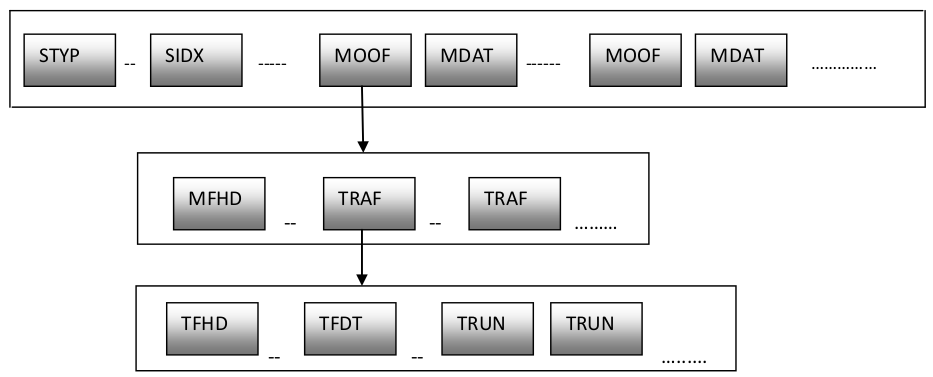
\includegraphics[width=12cm]{images/isobmff_boxes.png}
	\caption{Hierarchisch verschachtelte Boxen laut IBMFF, Quelle: \cite{mazhar_compliance_2011}, Figure 26, S. 50}
	\label{ibmff_boxes}
\end{figure}

MPEG-2 TS hingegen wurde für die Übertragung von Medienströmen über unsichere Medien (zB Broadcasts über Satellit) entworfen. Aufgrund der unsicheren Natur des Übertragungsmediums wird verstärkt Fokus auf Fehlerkorrektur und Synchronisation gelegt. MPEG-2 TS finden vorallem im Digitalfernsehen Anwendung und wird mitunter bei DVB und IPTV verwendet. MPEG-2 TS basierende Segmente verarbeiten \textit{Packets}, welche wiederum in \textit{Header} und \textit{Payload} unterteilt werden.

DASH unterscheidet zwischen verschiedenen Segmenttypen die je nach zugrundeliegendem Containerformat unterschiedlich strukturiert sind.

\subsubsection{Initialization Segments}
Das Initialisierungssegment beinhält keine kodierten Mediendaten sondern nur Metadaten die Aussagen über die Nutzdaten des zu verarbeitenden Medienstroms treffen \cite{international_organization_for_standardization_isoiec_nodate}. Mit diesen Metadaten sollte die verarbeitende Software in der Lage sein alle Folgesegmente richtig zu dekodieren.

IBMFF sieht eine Aufteilung des Initialisierungssegments in zwei Boxes vor. Eine \textit{File-Type}-Box (\attr{ftyp}) welche den Dateityp angibt und eine \textit{Movie}-Box (\attr{moov}) die Information über Anzeigecharakteristiken des Videos beinhält.

Initialisierungssegmente für MPEG-2 TS beinhalten Informationen die sich über den gesamten Strom hinweg nicht ändern. Dazu gehört in jedem Fall ein \attr{PAT}-Abschnitt (\textbf{P}rogram \textbf{A}ssociation \textbf{T}able) welcher Programmnummern für alle im Stream enthaltenen Programme beinhält. Häufig wird auch ein \attr{PMT} (\textbf{P}rogram \textbf{M}ap \textbf{T}able) inkludiert, welcher weitere Informationen zu den Programmen enthält. Es können auch noch weitere Abschnitte enthalten sein, solange sich die beinhalteten Daten über den gesamten Transportstrom hinweg nicht ändern.
Init-Segmente für MPEG-2 TS müssen nicht vollständig sein. D.h. es reicht wenn die Konkatenation aller Pakete des Stroms alle Metadaten beinhält die für das Abspielen nötig sind.

Initialisierungssegmente sind optional. Wird kein Initialisierungssegment an den Player übermittelt müssen die Mediensegmente \textit{selbstinitialisierend} sein.

\subsubsection{Media Segments}
Mediensegmente beinhalten die eigentlichen Mediendaten welche in den Initialisierungsdaten beschrieben sind und wiedergegeben werden können \cite{international_organization_for_standardization_isoiec_nodate}.

Im Fall von IBMFF wird zwischen vier Typen von Mediensegmenten unterschieden:

\begin{itemize}
	\item \textbf{Delivery Unit Media Segment} bilden die Grundlage für alle weiteren Segmenttypen. Jedes Segment besitzt eines oder mehrere \textit{Movie Fragments} die wiederum aus einer \attr{moof}- und einer \attr{mdat}-Box bestehen. Ersteres beinhält Metadaten über das Fragment, zweiteres beinhält die eigentlichen, kodierten Mediendaten. Movie Fragments müssen \textit{self-contained} sein. Das bedeutet dass keine Referenzen auf Daten außerhalb des eigenen Segments verwendet werden dürfen. Erkennbar sind Delivery Unit Media Segments an der \textit{Segment Type}-Box \attr{stype}, welche den Wert \attr{dums} aufweist.
	\item \textbf{Simple format type} ist über den \attr{styp} \attr{'msdh'} erkennbar und muss alle Anforderungen für ein Delivery Unit Segment erfüllen. Weiters können eine oder mehrere \attr{sidx}-Box(en) (Segment Index) vorhanden sein und vor der ersten \attr{moof}-Box platziert werden. Zudem muss jedes \textit{Track Fragment} (\attr{traf}) eine \textit{Track Fragment Decode Time} (\attr{tfdt}) enthalten.
	\item \textbf{Indexed Media Segment}s können über den \attr{stype} \attr{'msix'} identifiziert werden und basieren ebenfalls auf den Vorgaben für Delivery Unit Segmente. Zudem wird jede \attr{moof}-Box direkt von der zugehörigen \attr{mdat}-Box gefolgt. Die Präsenz von \attr{sidx}-Boxen wie im \textit{Simple format type} ist nicht optional.
	\item \textbf{Random Access Media Segment}s erfüllen die Anforderung des \textit{Simple format type}s und beinhalten genug Information (zB Verschlüsselungsinformation) um in Kombination mit dem Initialisierungssegment den Medienstrom wiedergeben zu können. Sie können also wahlfrei (\textit{random}) abgespielt werden.
\end{itemize}

MPEG-2 TS unterscheidet grundsätzlich nur zwischen zwei Typen von Mediensegmenten:
\begin{itemize}
	\item Ein \textbf{Basic Media Segment} besteht nur aus vollständigen MPEG-2 TS Paketen in denen genau ein Programm definiert ist und darf nicht von Initialisierungsinformation abhängig sein, die erst in darauffolgenden Segmenten verfügbar ist. \textit{Basic Media Segments} können außerdem selbstinitialiserend sein und/oder Information zur Verschlüsselung von Folgepaketen beinhalten.
	\item \textbf{Bitstream Switching Segment}s sollen keine Mediendaten beinhalten. Sie werden verwendet wenn der jeweilige Player auf eine \elem{Representation} wechselt die abweichende Initialisierungsdaten beinhält. In diesem Fall werden die Initialisierungsinformationen aus den Switching-Segmenten gewonnen.
\end{itemize}

Mediendaten können nicht abgespielt werden solange das Initialisierungssegment nicht heruntergeladen und verarbeitet wurde was die Vorlaufzeit für den Beginn des Playbacks negativ beeinträchtigt. Aus diesem Grund wurden selbstinitialisierende Mediensegmente eingeführt, die an ihrem \attr{ftyp} 'dsms' erkennbar sind. Die Abkürzung steht für \textit{DASH Self-Initializing Media Segment}.

\subsubsection{Index Segments}
Indexsegmente enthalten Indexinformation über die Mediensegmente des Streams und werden unabhängig vom zugrundeliegenden Format des Streams als Sequenz vom IBMFF-Boxen repräsentiert. Für die Zusammenarbeit in MPEG-2 TS existieren Box-Typen die speziell für diesen Fall geschaffen wurden \cite{international_organization_for_standardization_isoiec_nodate}.
Mithilfe eines Indexsegments kann effizient auf darauffolgende Mediensegmente zugegriffen werden. Das wird mithilfe der Angabe von Byte-Offsets in Verbindung mit dem jeweiligen Segment-Index (\attr{sidx}) erreicht.

Ein Indexsegment kann entweder ein einzelnes Mediensegment oder alle Segmente einer \elem{Representation} indexieren.

Jedes Mediensegment kann außerdem einen Segment-Index besitzen. IBMFF realisiert dies mithilfe einer dediziert \attr{sidx}-Box. MPEG-2 TS nutzt den \attr{PID}-Wert (\textbf{P}rogram \textbf{ID}) für den Segment Index. 

\subsection{Media Presentation Timeline}
Ein zentrales Konzept in DASH ist die \textit{Media Presentation Timeline}. Dabei handelt es sich um eine globale, innerhalb einer MPD gültige Timeline die Synchronisation von verschiedenen Medienkomponenten erleichtert. Sämtliche Komponenten in allen potentiell unterschiedlich kodierten Versionen orientieren sich an dieser Timeline \cite{international_organization_for_standardization_isoiec_nodate}.

Durch dieses Modell müssen Elemente nicht mehr mit einer aufsteigenden ID versehen werden um in der korrekten Reihenfolge abgespielt werden zu können. Stattdessen werden die Segmente mit timestamps versehen, die Segmentpositionen an der globalen Media Presentation Timeline festlegen.

\subsection{Profile}
\label{profiles}
DASH unterstützt unterschiedliche Profile mit deren Hilfe Rückschluss auf verwendete Features geschlossen werden kann \cite{international_organization_for_standardization_isoiec_nodate}. Die unterstützten Profile können im MPD-Root-Tag als kommaseparierte Liste aufgeführt werden.

Je nach Profil existieren unterschiedliche Restriktionen im Bezug auf MPD und Segmentformate welche für alle angegebenen Profile erfüllt sein müssen um als valide zu gelten.

Profile können wieder je nach zugrundeliegendem Containerformat in zwei Kategorien eingeteilt werden. (IBMFF oder MPEG-2 TS)

\begin{itemize}
	\item \textbf{Full (\attr{urn:mpeg:dash:profile:full:2011})}: Alle Features und Segmenttypen des Standards werden unterstützt. Alle weiteren Profile unterstützen eine Teilmenge der Features die vom \textit{full}-Profil umfasst werden.
	\item \textbf{IBMFF On Demand (\attr{urn:mpeg:dash:profile:isoff-on-demand:2011})}: On-Demand Medien liegen zum Zeitpunkt des Abrufs bereits vollständig vor. D.h. dass im Gegensatz zu Live-Medien kein Inhalt mehr zusätzlich generiert wird. Haupteinschränkung in diesem Profil ist, dass \elem{Representation}s nur durch ein einziges Segment dargestellt werden dürfen. Dadurch wird die Verwendung von \elem{SegmentList} und \elem{SegmentTemplate} ausgeschlossen. Das \attr{type}-Attribut in \elem{MPD} muss außerdem den Wert \attr{'static'} aufweisen. Genauere Ausführungen können im Standard nachgelesen werden.
	\item \textbf{IBMFF Live (\attr{urn:mpeg:dash:profile:isoff-live:2011)}}: Um die Latenz für den Live-Einsatz möglichst niedrig zu halten, werden Segmente von sehr kurzer Dauer erzeugt. Diese lassen sich schneller kodieren. Außerdem wird empfohlen innerhalb der MPD ein \elem{SegmentTemplate} zu verwenden. Ansonsten muss vor jedem Segment-Request auch die MPD upgedated werden. Weiters wird die Verwendung von Indexsegmenten ausgeschlossen. Alle Mediensegmente müssen also selbstinitialisierend sein.
	\item \textbf{MPEG-2 TS main (\attr{urn:mpeg:dash:profile:mp2t-main:2011})}: Verwendete Elemente der MPD und Segmentformate werden, mit Ausnahme der Verwendung von MPEG-2 TS statt IBMFF, nur sehr gering eingeschränkt. \elem{Representation}s die ein \elem{SegmentTimeline}-Element beinhalten werden ignoriert. Die Verwendung von Indexsegmenten wird stark empfohlen.
	\item \textbf{MPEG-2 TS simple (\attr{urn:mpeg:dash:profile:mp2t-simple:2011})}: Ziel dieses Profils ist es, die Implementierung des Wechsels zu einer anderen \elem{Representation} zu vereinfachen. Das wird erreicht indem die Segmentstruktur stärker eingeschränkt wird. Software nach ISO/IEC 13818-1 (Generic coding of moving pictures and associated audio) sollte in der Lage sein den Stream durch Konkatenation aller Segmente verschiedener \elem{Representation}s im selben \elem{AdaptationSet} wiederzugeben. PSI (Program specific metadata), welche mitunter PMT und PAT enthält, muss dafür in allen \elem{Representation}s identisch sein. Die Verwendung von Indexsegmenten und \elem{SegmentTemplate} werden zudem stark empfohlen.
\end{itemize}
 
Für Broadcast-TV existiert zudem ein eigenes, auf IBMFF basierendes Profil. Ebenfalls existieren zum \textit{Live}- und \textit{On-Demand}-Profil \textit{extended} Versionen die unterstützte Features weniger stark einschränken. Diese können bei Bedarf im Standard nachgelesen werden.

\section{Technologien rund um MPEG-DASH}
Um MPEG-DASH funktionstüchtig und messbar für den praktischen Einsatz zu machen, bedarf es einiger Technologien die nicht konkret im oder durch den Standard definiert werden. Auf diese Technologien, welche mitunter für Übertragung und Bitratenadaptierung zuständig sind, wird im Folgenden überblicksmäßig eingegangen.

\subsection{HTTP für Videostreaming}
Bisher wurde stark darauf eingegangen, welchen Standards Clients und Server im Streamingprozess zu folgen haben. Zur Kommunikation zwischen den beiden Instanzen sind jedoch Netzwerkprotokolle zuständig.

Bevor adaptives Streaming und HTTP für Videostreaming über das Internet benutzt wurden, war das Real-Time Streaming Protocol (RTSP) vorherrschend im Videostreaming-Sektor \cite{stockhammer_dynamic_2011}. RTSP speichert und verwaltet den Status jedes verbundenen Clients auf der Serverseite und zählt deshalb zur Gattung der zustandsorientierten Protokolle. Das reduziert zwar clientseitigen Aufwand, bringt aber eine Reihe von Problemen mit sich. Mit steigendem Videoverkehr werden immer leistungsstärkere Server benötigt, um alle Clients zeitgerecht bedienen zu können \cite{stockhammer_dynamic_2011}. Zudem sind Skalierbarkeit weder im Sinne von High-Performance noch beim Failover trivial, da der Zustand des Clients \textit{übertragen} werden muss.

HTTP hingegen ist ein zustandsloses Protokoll. Das bedeutet, dass jede Anfrage eines Clients komplett unabhängig von etwaigen vorhergehenden Anfragen behandelt wird. Durch diese Eigenschaft ist HTTP von Natur aus gut skalierbar. Zusätzlich unterstützt wird die Skalierbarkeit durch den Einsatz von Content Distribution Networks (CDNs), die als Proxys den ursprünglichen HTTP-Server entlasten und zusätzlich bessere Latenz durch Ausnutzung geographischer Faktoren versprechen \cite{buyya_content_2008}.

Skalierbarkeit ist allerdings nicht der einzige Grund für den Einsatz von HTTP im Streamingbereich, wie Stockhammer in \cite{stockhammer_dynamic_2011} aufzeigt. Einige andere wären: 

\begin{itemize}
	\item Streaming über HTTP vermeidet weitgehend Probleme mit NAT und Firewalls.
	\item Standard-HTTP-Server (und Caches) sind weit verbreitet und deshalb günstig.
	\item Durch die Zustandslosigkeit von HTTP kann die Kontrolle über den Streamingprozess komplett an den Client übergeben werden. Bei Änderungen der Bandbreite und Wechsel auf eine höhere/niedrigere Bitrate ist keine Verhandlung (eng. \textit{negotiation}) mit dem Server nötig.
\end{itemize}

Der Download von Segmenten über den Client erfolgt über HTTP GET-Requests. Um auch \textit{partielle GET-Requests} für Byte-Ranges benutzen zu können, schreibt DASH die Verwendung von HTTP/1.1 vor \cite{international_organization_for_standardization_isoiec_nodate}.
Damit lassen sich Teile von Resourcen anfragen und herunterladen, was speziell bei großen Dateien sinnvoll sein kann. Die Angabe der benötigten Bytes erfolgt dabei im \textit{Range}-Feld des HTTP-Headers. Der Server kann daraufhin mit einem Status-Code \textit{206 Partial Content} die angefragten Daten liefern, oder mit \textit{416 Requested Range Not Satisfiable} angeben, dass die angefragte Byte-Range nicht valide ist. \cite{krishnamurthy_key_1999}

\subsection{Algorithmen zur Bitratenadaptierung}
Eine weitere Zuständigkeit des Clients ist die Steuerung der Bitratenadaption. Der implementierte Algorithmus ist dafür zuständig, wann auf eine andere \elem{Representation} mit niedrigerer Bitrate (schlechtere Qualität) oder höherer Bitrate (bessere Qualität) gewechselt wird.

Dieser Mechanismus ist im Gegensatz zur MPD-Struktur und den Segmentformaten nicht im Standard enthalten und deshalb implementierungsspezifisch in Bezug auf den verwendeten Client.

Diese Algorithmen wurden von Bentaleb et al. \cite{bentaleb_survey_2019} in vier Kategorien unterteilt:

\begin{enumerate}
	\item \textbf{Client-based adaptation}: Der Großteil aller Bitratenadaptierungsschemen findet auf der Clientseite statt. Ein Teil der Clientsoftware misst ständig Metriken wie die verfügbare Bandbreite, Pufferstand oder CPU-Auslastung und entscheidet basierend darauf, welches Segment als nächstes heruntergeladen wird. 
	\item \textbf{Server-based adaptation}: Server-basierte Ansätze zur Bitratenadaptierung beziehen den Client nicht mit ein, sondern entscheiden via \textit{traffic-shaping}, welcher Client wie viel Videobitrate (Qualität) erhält. Damit möchte man einer unfairen Verteilung der Netzwerkressourcen zwischen Clients und Bitraten-Instabilität vermeiden. Letzteres tritt auf, wenn der Client die Bitrate oft ändert und es dadurch zu Qualitätsschwankungen kommt. Da dafür aber Zusatzsoftware am Server benötigt wird, stehen serverseitige Ansätze im Konflikt mit dem DASH-Standard. Dieser besagt, dass die Auslieferung der Segmente über einen Standard-HTTP-Server erfolgt.
	\item \textbf{Network-assisted adaptation}: Dieser Ansatz ermöglicht es den Clients, Netzwerkinformationen bei der Auswahl der Bitrate miteinzubeziehen. Um an diese Netzwerkdaten zu kommen, muss ein \textit{Agent} im Netzwerk platziert werden, der Clients über die effizienteste Nutzung der vorhandenen Netzwerkressourcen informiert.
	\item \textbf{Hybrid adaptation}: Bei hybriden Verfahren werden mehrere Komponenten in Verbindung miteinander eingesetzt, um \textit{Quality of Experience} (QoE) für den Benutzer zu erhöhen. Rein clientbasierte Ansätze stoßen an ihre Grenzen, wenn mehrere DASH-Clients über ein gemeinsames Netzwerk streamen, da ein Client für sich keinen Überblick über die Gesamtsituation im Netzwerk hat. \textit{Software Defined Networks} (SDNs) verwenden ohnehin einen Controller für die Verwaltung der Netzwerkgeräte und Ressourcen. Dieser kann über ein QoE-Fairness-Framework (QFF) sicherstellen, dass die verfügbaren Ressourcen gleichmäßig zwischen den Clients aufgeteilt werden. Ein weiterer Hybridansatz ist \textit{Server and Network-assisted DASH (SAND)} \cite{stockhhammer_sand}. SAND bezieht Server und Netzwerkmetriken mit ein die einerseits an die Clients verteilt und ebenso an \textit{DASH Aware Network Elements (DANE)} gesendet werden. Die gesammelten Metriken fließen in die Entscheidung des Clients ein, während DANEs die Bereitstellung dynamisch optimieren.
\end{enumerate}

\subsection{Quality of Experience (QoE)}
Oberstes Ziel von adaptiven Streamingtechnologien ist erhöhte Benutzerzufriedenheit. Um Benutzerzufriedenheit mit einem System (nicht nur DASH) konzeptuell darstellen zu können, wurde der Begriff \textit{Quality of Experience (QoE)} wie folgt definiert:

\glqq \textit{Quality of Experience (QoE) is the degree of delight or annoyance of the user of an application or service. It results from the fulfillment of his or her expectations with respect to the utility and / or enjoyment of the application or service in the light of the user’s personality and current state.}\grqq \cite{brunnstrom_qualinet_2013}

Durch den Einbezug der Persönlichkeit und Befindlichkeit eines Benutzers / einer Benutzerin während der Nutzung des Systems grenzt sich QoE vom verbreiteten Konzept der \textit{Quality of Service (QoS)} ab. QoS wird weitgehend für die Charakterisierung von Telekommunikationssystemen und deren Fähigkeit, den Anforderungen von BenutzerInnen und Diensten gerecht zu werden, verwendet. Schlechte QoS impliziert schlechte QoE. Gute QoS allerdings reicht nicht aus, um auch gute QoE zu garantieren \cite{brunnstrom_qualinet_2013}.

Seufert et al. \cite{seufert_survey_2015} unterteilt QoE-Einflussfaktoren in DASH-Streams in drei Kategorien:
\begin{itemize}
	\item \textbf{Initial Delay} nennt man die Zeit, die verstreicht, bis ein Multimedia-Client mit dem Playback beginnen kann. Diese Verzögerung zu Beginn des Streamingprozesses entsteht, da initial der Puffer des Clients gefüllt werden muss. Diese Wartezeit beeinflusst die QoE nur in geringem Ausmaß. 90\% der NutzerInnen geben an, dass sie Wartezeiten zu Beginn des Videos einer Unterbrechung des laufenden Playbacks (\textit{Stalling}) bevorzugen. Anders verhält sich dieser Parameter, wenn viele, kurze Videos nur zu Teilen konsumiert werden (\textit{Video Browsing}).
	\item Als \textbf{Stalling} bezeichnet man einen Stopp des Videoplaybacks aufgrund von Pufferleerläufen. Wenn der clientseitige Puffer leer ist, muss die Wiedergabe gestoppt werden, um diesen wieder mit Mediendaten zu füllen. Dieser Vorgang wird \textit{Rebuffering} genannt. Die Größe des Puffers spielt hierbei eine zentrale Rolle. Bei großen Puffern wird die Wahrscheinlichkeit von Stallings minimiert, während allerdings die Dauer eines Rebuffering-Events zunimmt. Testpersonen gaben Stalling als den Faktor an der das Streamingerlebnis am stärksten negativ beeinflusst. Weniger, längere Stallings werden häufigeren, kurzen Rebufferings bevorzugt. 
	\item Durch \textbf{Adaption} kann die Qualitätsstufe des konsumierten Mediums während der Wiedergabe gewechselt werden. Diese, im klassischen Videostreaming nicht vorhandene Dimension wird von Testpersonen besonders bei häufigen Qualitätswechseln als störend empfunden. Adaptation degradiert die QoE trotzdem weniger schwer als Stalling.
\end{itemize}

Insgesamt verbessert adpatives Streaming die QoE gegenüber klassischem Streaming stark. Wie in \cite{yao_empirical_2011}, gezeigt wird Stalling, welches als größter Störeinfluss für QoE gilt, durch Bitratenadaption um bis zu 80\% reduziert. Im Laufe der Erforschung von QoE in DASH-Streams konnte eine starke Korrelation zwischen QoE und der verwendeten Puffer- sowie Segmentgröße gefunden werden \cite{seufert_survey_2015}.

\subsection{Tools und Referenzsoftware}
Um Performancemessungen in eigenen DASH-Streams durchführen zu können und diese in Beziehung mit QoE-Parametern zu stellen, existiert eine Reihe von frei zugänglichen Softwareprodukten.

Grundlage für die Realisierung eines DASH-Clients bietet die offizielle Referenzbibliothek \textit{libdash}. Wie in Grafik \ref{libdash_embedded} dargestellt besteht die Bibliothek aus dem MPD Parser, der für die Verarbeitung der MPD zuständig ist, und dem HTTP-Manager, der sich um das Herunterladen der Segmente kümmert. Um libdash in eigenen Applikationen einzubinden, wird eine objektorientierte Schnittstelle angeboten.

\begin{center}
	\begin{figure}[ht]
		\centering
		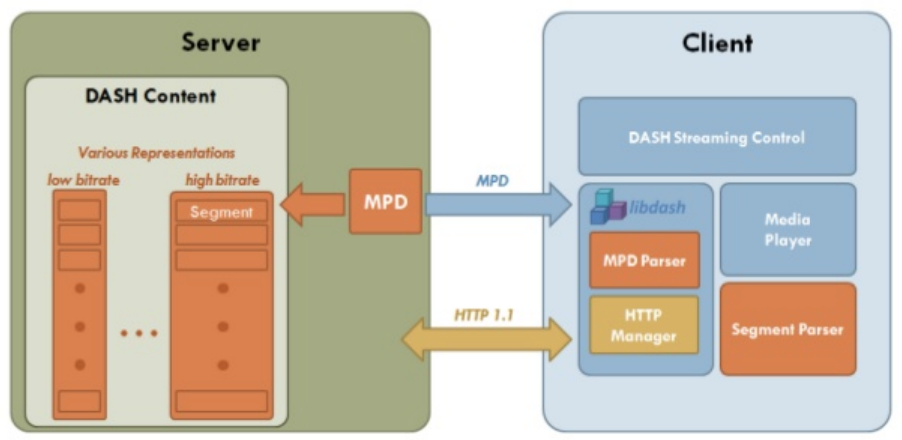
\includegraphics[width=12cm]{images/libdash_embedded.png}
		\caption{Rolle von libdash im Streamingprozess, Quelle: \hyperref{https://doi.org/10.1109/CAIS.2019.8769444}{}{}{Implementation of QoE Model Based on Pixel Density}}
		\label{libdash_embedded}
	\end{figure}
\end{center}

Das DASH-Industry-Forum (kurz \textit{DASH-IF}) bietet auf seiner Website\footnote{\url{https://dashif.org/software/}} einen Überblick über aktuelle Referenzsoftware. Einen vollständig implementierten, webbassierten DASH-Player\footnote{\url{https://bitmovin.com/demos/stream-test}} bietet auch die Firma Bitmovin an. Dieser ermöglicht das Testen von DASH adaptiven und progressiven Streams in verschiedenen Konfigurationen. Weiter werden Pufferstand sowie Bitrate des Videos aufgzeichnet und graphisch dargestellt.

Serverseitig kann Standard HTTP-Server-Software zur Auslieferung der Segmente wie beispielsweise \textit{nginx} oder \textit{Apache HTTP Server} verwendet werden. Die Generierung von DASH-konformen Segmentdateien und MPDs kann mit dem Tool \hyperref{https://github.com/gpac/gpac}{}{}{mp4box}\footnote{\url{https://github.com/gpac/gpac/wiki/MP4Box}} durchgeführt werden. Mp4Box ist Teil des GPAC-Projekts, welches OpenSource-Tools für verschiedenste Multimediadomänen anbietet.

Auf der Website des DASH-IFs können IBMFF-Segmente und MPD-Dateien mithilfe des \hyperref{https://conformance.dashif.org/}{}{}{Conformance-Tools}\footnote{\url{https://conformance.dashif.org/}} kostenlos validiert und getestet werden.

\section{Konklusion}
HTTP Adaptive Streaming (HAS) ist aus der modernen Medienlandschaft nicht mehr wegzudenken und hat mit MPEG-DASH einen offenen und gut unterstützten Standard erhalten. Im Verlauf dieser Seminararbeit haben wir uns mit den im Standard definierten Bausteinen von DASH, namentlich der Media Presentation Description und den Segmentformaten auseinandergesetzt um ein Grundverständnis für deren Zusammenspiel zu schaffen.

Anschließend wurde ein Überblick über verschiedene Arten von Algorithmen zur Bitraten-Adaption sowie Quality of Experience geboten. Abschließend folgte eine Vorstellung von verschiedenen Werkzeugen die den Leser dazu befähigen sollen, selbst DASH-Streams zu erzeugen, zu validieren und deren Performance zu messen.

% % % % % % % % % % % % % % % % % % % % % %

% % % % % % % % % % % % % % % % % % % % % % 
% Literaturverzeichnis
% % % % % % % % % % % % % % % % % % % % % %
\newpage
\printbibliography
\end{document}

% % % % % % % % % % % % % % % % % % % % % %